\newpage
\lecture{11}{Измеримые пространства.}

\subsection{Борелевские функции.}

\textit{Напоминание:} функция $f:\:\R\to\R$ непрерывна $\Leftrightarrow$ $f^{-1}(U)$ открыто
для любого открытого множества $U\subset\R$, где $f^{-1}(U) = \{x\in\R:\: f(x)\in U\}$~---
полный прообраз $U$.

\begin{definition}
    Функция $f:\: \R\to\R$ называется \mdef{борелевской} (измеримой по Борелю),
    если $\forall$ открытого $U\subset\R$ выполняется $f^{-1}(U)\in\CB(\R)$.
\end{definition}

\begin{exercise}
    Существуют борелевские \textbf{не} непрерывные функции, например,
    \[
        f(x)=\sign x = \begin{cases}
            1,  & x>0, \\
            0,  & x=0, \\
            -1, & x<0. \\
        \end{cases}
    \]
\end{exercise}

\begin{definition}
    Введем \mdef{индикаторную функцию} (\mdef{индикатор} множества $A$):
    \[
        1_A(x)=\begin{cases}
            1, & x\in A,    \\
            0, & x\notin A.
        \end{cases}
    \]

    \begin{remark}
        Данный объект часто называют \mdef{характеристической функцией}, но
        так как в теории вероятности под этим подразумевается немного другая вещь, будем придерживаться
        данного определения.
    \end{remark}
\end{definition}

\begin{claim}
    $\forall B\in\CB(\R)\ 1_B$~--- борелевская функция.
\end{claim}

\begin{remark}
    Аналогичные определения можно дать для функций вида $f:\: X\to Y$, где
    $X$ и $Y$~--- метрические пространства.
\end{remark}

\subsection{Измеримые пространства.}

\begin{definition}
    Пусть $X$~--- множество, $\CE\subset\CP(X)$~--- $\sigma$"=алгебра.
    Тогда пара $(X,\, \CE)$ называется измеримым пространством.
\end{definition}

\begin{exercise}
    В качестве $X$ можем взять $\R$, а $\CE=\CB(\R)$ или $\CE=\mathfrak{m}(\R)=\{A\subset\R:\
        A\text{ измеримо по Лебегу}\}$.
\end{exercise}

\begin{remark}
    На первый взгляд обе сигма-алгебры подозрительно похожи, но
    можно выделить два утверждения:
    \begin{enumerate}
        \item $\CB(\R)\subset\mathfrak{m}(\R)$,
        \item $\forall A\in\mathfrak{m}(\R)\ \exists N\subset \R:\
                  m^*(N)=0:\ \exists B\in\CB(\R)$ и $A=B\sqcup N$, где $m^*$~--- внешняя мера Лебега.
    \end{enumerate}
\end{remark}

\begin{definition}
    Пусть $(X,\, \CE)$ и $(Y,\, \F)$~--- измеримые пространства. Функцию $f:\: X\to Y$
    будем называть \mdef{измеримой} относительно пары $(\CE,\, \F)$, если
    $\forall A\in\F$ выполнено $f^{-1}(A)\in\CE$.

    Если $Y=\R$ и $\F=\CB(\R)$ (или $Y=\overline{\R}$ и $\F=\CB(\overline{\R})$) и
    $f$ измерима относительно $(\CE,\, \F)$, то будем говорить, что $f$ \mdef{измерима}
    относительно $\CE$.
\end{definition}

\begin{claim}
    Пусть $\CG\subset\CP(Y)$, $f:\: X\to Y$. Тогда $f$ измерима относительно $(\CE,\, \sigma(\CG))$
    тогда и только тогда, когда $\forall A\in\CG$ выполнено $f^{-1}(A)\in\CE$.

    \begin{proof}

        \circled{$\Rightarrow$} Следует сразу из того, что $\CG\subset \sigma(\CG)$.

        \circled{$\Leftarrow$} Пусть $\CM:=\{A\in\F:\: f^{-1}(A)\in\CE\}$, где $\F=\sigma(\CG)$. По условию
        $\CG\subset\CM$. Если доказать, что $\CM$~--- $\sigma$"=алгебра, тогда из $\CG\subset\CM$
        следует $\sigma(\CG)\subset\CM$.

        Итак, докажем, что $\CM$~--- $\sigma$"=алгебра.
        \begin{enumerate}
            \item $\varnothing \in\CM$, так как $f^{-1}(\varnothing)=\varnothing\in\CE$.
            \item $\forall A\in\CM\ A^C\in\CM$, так как
                  \[
                      f^{-1}(A^C)=\{x\in X:\: \underbrace{f(x)\in A^C}_{f(x)\notin A}\}=
                      X\setminus\left\{x\in X:\: f(x)\in A\right\}=f^{-1}(A)^C.
                  \]
                  То есть:
                  \[
                      A\in\CM\Rightarrow f^{-1}(A)\in\CE\Rightarrow \left(f^{-1}(A)\right)^C\in\CE\Rightarrow
                      f^{-1}\left(A^C\right)\in\CE.
                  \]
            \item Пусть $A_n\in\CM\ \forall n\in\N$. Тогда
                  \[
                      f^{-1}\left(\bigcup_{n=1}^{\infty}A_n\right)=\left\{x\in X:\: \exists n\in \N\ f(x)\in A_n\right\}
                      =\bigcup_{n\in\N}\left\{x\in X:\: f(x)\in A_n\right\}=\bigcup_{n=1}^{\infty}f^{-1}(A_n).
                  \]
                  Далее
                  \[
                      A_n\in\CM\Rightarrow f^{-1}\in\CE\Rightarrow\bigcup_{n=1}^{\infty}f^{-1}(A_n)\in\CE.
                  \]
        \end{enumerate}

    \end{proof}
\end{claim}

\begin{next0}
    Функция $f:\:\R\to\R$ является борелевской тогда и только тогда, когда $f$ измерима относительно
    $\CB(\R)$.
\end{next0}

\begin{definition}
    Функцию $f:\:\R\to\R$ будем называть \mdef{измеримой по Лебегу}, если она измерима
    относительно $\mathfrak{m}(\R)$.
\end{definition}

Приведем пример не измеримой по Лебегу функции.

\begin{exercise}
    Пусть $V\subset \R$~--- множество Витали (или любое другое множество не измеримое по Лебегу).
    Тогда $1_V$ является не измеримой по Лебегу функцией,
    так как $\{1\}$~--- борелевское, но $1_V^{-1}(\{1\})=V\notin\mathfrak{m}(\R)$.
\end{exercise}

\begin{remark}
    $\overline{\R}=\R\cup\{\pm\infty\}$~--- метрическое пространство, если расстояние определить следующим образом:
    рассмотрим функцию $f(t) = \arctan(t)$, доопределим ее в $\pm\infty$: $\arctan(\pm\infty)=\pm\dfrac{\pi}{2}$.
    \begin{figure}[!ht]
        \centering
        \tikzset{every picture/.style={line width=0.75pt}} %set default line width to 0.75pt        

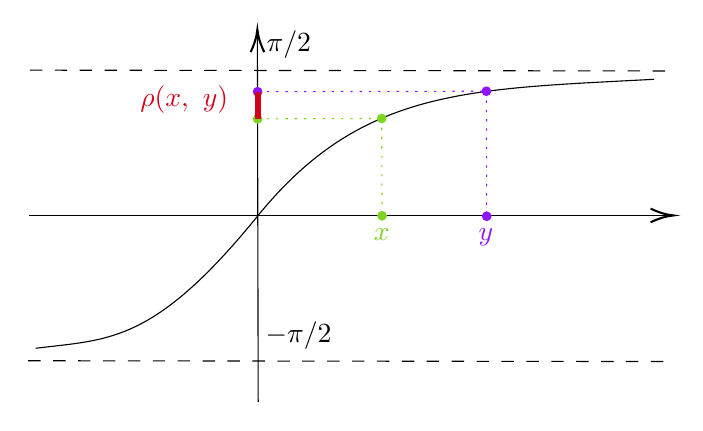
\begin{tikzpicture}[x=0.75pt,y=0.75pt,yscale=-1,xscale=1]
%uncomment if require: \path (0,300); %set diagram left start at 0, and has height of 300

%Straight Lines [id:da01253990328815191] 
\draw    (120.04,259.96) -- (119.64,82.36) ;
\draw [shift={(119.64,80.36)}, rotate = 449.87] [color={rgb, 255:red, 0; green, 0; blue, 0 }  ][line width=0.75]    (10.93,-3.29) .. controls (6.95,-1.4) and (3.31,-0.3) .. (0,0) .. controls (3.31,0.3) and (6.95,1.4) .. (10.93,3.29)   ;
%Straight Lines [id:da011511383436563216] 
\draw    (9.64,169.96) -- (318.04,169.96) ;
\draw [shift={(320.04,169.96)}, rotate = 180] [color={rgb, 255:red, 0; green, 0; blue, 0 }  ][line width=0.75]    (10.93,-3.29) .. controls (6.95,-1.4) and (3.31,-0.3) .. (0,0) .. controls (3.31,0.3) and (6.95,1.4) .. (10.93,3.29)   ;
%Straight Lines [id:da3525055949245628] 
\draw  [dash pattern={on 4.5pt off 4.5pt}]  (9.24,239.96) -- (319.64,240.36) ;
%Straight Lines [id:da9013132184394284] 
\draw  [dash pattern={on 4.5pt off 4.5pt}]  (10.04,99.96) -- (320.44,100.36) ;
%Curve Lines [id:da28618381116787295] 
\draw    (12.84,233.96) .. controls (48.04,229.56) and (69.64,231.96) .. (119.84,170.16) .. controls (170.04,108.36) and (221.64,109.16) .. (310.84,104.36) ;
%Flowchart: Connector [id:dp9476639517392225] 
\draw  [color={rgb, 255:red, 126; green, 211; blue, 33 }  ,draw opacity=1 ][fill={rgb, 255:red, 126; green, 211; blue, 33 }  ,fill opacity=1 ] (177.64,170.12) .. controls (177.64,168.99) and (178.56,168.07) .. (179.7,168.07) .. controls (180.84,168.07) and (181.76,168.99) .. (181.76,170.12) .. controls (181.76,171.26) and (180.84,172.18) .. (179.7,172.18) .. controls (178.56,172.18) and (177.64,171.26) .. (177.64,170.12) -- cycle ;
%Flowchart: Connector [id:dp5108999664707425] 
\draw  [color={rgb, 255:red, 144; green, 19; blue, 254 }  ,draw opacity=1 ][fill={rgb, 255:red, 144; green, 19; blue, 254 }  ,fill opacity=1 ] (228.09,170.34) .. controls (228.09,169.21) and (229.01,168.29) .. (230.14,168.29) .. controls (231.28,168.29) and (232.2,169.21) .. (232.2,170.34) .. controls (232.2,171.48) and (231.28,172.4) .. (230.14,172.4) .. controls (229.01,172.4) and (228.09,171.48) .. (228.09,170.34) -- cycle ;
%Straight Lines [id:da760850287045677] 
\draw [color={rgb, 255:red, 126; green, 211; blue, 33 }  ,draw opacity=1 ] [dash pattern={on 0.84pt off 2.51pt}]  (179.53,123.22) -- (179.7,170.12) ;
%Straight Lines [id:da492720321335101] 
\draw [color={rgb, 255:red, 144; green, 19; blue, 254 }  ,draw opacity=1 ] [dash pattern={on 0.84pt off 2.51pt}]  (229.98,110.11) -- (230.14,170.34) ;
%Flowchart: Connector [id:dp10875556229828831] 
\draw  [color={rgb, 255:red, 126; green, 211; blue, 33 }  ,draw opacity=1 ][fill={rgb, 255:red, 126; green, 211; blue, 33 }  ,fill opacity=1 ] (177.48,123.22) .. controls (177.48,122.09) and (178.4,121.17) .. (179.53,121.17) .. controls (180.67,121.17) and (181.59,122.09) .. (181.59,123.22) .. controls (181.59,124.36) and (180.67,125.28) .. (179.53,125.28) .. controls (178.4,125.28) and (177.48,124.36) .. (177.48,123.22) -- cycle ;
%Flowchart: Connector [id:dp7021743431110545] 
\draw  [color={rgb, 255:red, 144; green, 19; blue, 254 }  ,draw opacity=1 ][fill={rgb, 255:red, 144; green, 19; blue, 254 }  ,fill opacity=1 ] (227.92,110.11) .. controls (227.92,108.98) and (228.84,108.06) .. (229.98,108.06) .. controls (231.11,108.06) and (232.03,108.98) .. (232.03,110.11) .. controls (232.03,111.25) and (231.11,112.17) .. (229.98,112.17) .. controls (228.84,112.17) and (227.92,111.25) .. (227.92,110.11) -- cycle ;
%Straight Lines [id:da939770188361363] 
\draw [color={rgb, 255:red, 126; green, 211; blue, 33 }  ,draw opacity=1 ] [dash pattern={on 0.84pt off 2.51pt}]  (119.76,123.44) -- (179.53,123.22) ;
%Straight Lines [id:da4619329715302538] 
\draw [color={rgb, 255:red, 144; green, 19; blue, 254 }  ,draw opacity=1 ] [dash pattern={on 0.84pt off 2.51pt}]  (119.76,110.33) -- (229.98,110.11) ;
%Flowchart: Connector [id:dp042464638370279806] 
\draw  [color={rgb, 255:red, 126; green, 211; blue, 33 }  ,draw opacity=1 ][fill={rgb, 255:red, 126; green, 211; blue, 33 }  ,fill opacity=1 ] (117.7,123.44) .. controls (117.7,122.31) and (118.62,121.39) .. (119.76,121.39) .. controls (120.89,121.39) and (121.81,122.31) .. (121.81,123.44) .. controls (121.81,124.58) and (120.89,125.5) .. (119.76,125.5) .. controls (118.62,125.5) and (117.7,124.58) .. (117.7,123.44) -- cycle ;
%Flowchart: Connector [id:dp02167511075412154] 
\draw  [color={rgb, 255:red, 144; green, 19; blue, 254 }  ,draw opacity=1 ][fill={rgb, 255:red, 144; green, 19; blue, 254 }  ,fill opacity=1 ] (117.7,110.33) .. controls (117.7,109.2) and (118.62,108.28) .. (119.76,108.28) .. controls (120.89,108.28) and (121.81,109.2) .. (121.81,110.33) .. controls (121.81,111.47) and (120.89,112.39) .. (119.76,112.39) .. controls (118.62,112.39) and (117.7,111.47) .. (117.7,110.33) -- cycle ;
%Straight Lines [id:da8116856549463478] 
\draw [color={rgb, 255:red, 208; green, 2; blue, 27 }  ,draw opacity=1 ][line width=2.25]    (119.76,110.33) -- (119.76,123.44) ;

% Text Node
\draw (122.84,79.76) node [anchor=north west][inner sep=0.75pt]   [align=left] {$\displaystyle \pi /2$};
% Text Node
\draw (122.34,219.76) node [anchor=north west][inner sep=0.75pt]   [align=left] {$\displaystyle -\pi /2$};
% Text Node
\draw (62,106) node [anchor=north west][inner sep=0.75pt]  [color={rgb, 255:red, 208; green, 2; blue, 27 }  ,opacity=1 ] [align=left] {$\displaystyle \rho ( x,\ y)$};
% Text Node
\draw (174.5,175) node [anchor=north west][inner sep=0.75pt]  [color={rgb, 255:red, 126; green, 211; blue, 33 }  ,opacity=1 ] [align=left] {$\displaystyle x$};
% Text Node
\draw (225,175) node [anchor=north west][inner sep=0.75pt]  [color={rgb, 255:red, 126; green, 211; blue, 33 }  ,opacity=1 ] [align=left] {$\displaystyle \textcolor[rgb]{0.56,0.07,1}{y}$};

\end{tikzpicture}
        \caption{Способ задать расстояние в $\overline{\R}$.}
        \label{fig:lect11:atan}
    \end{figure}
    Тогда расстояние между любыми двумя точками $x,\, y\in\overline{\R}$ определим как
    \[
        \rho(x,\, y) = |\arctan(x) - \arctan(y)|\quad \text{(см. рис. \ref{fig:lect11:atan})}
    \]

    Пусть тогда
    \[
        \tau_{\overline{\R}}:=\left\{U\subset\overline{\R}:\: \forall x\in U\ \exists r>0:\: \forall
        y\in\R:\: \rho(x,\, y)<r\Rightarrow y\in U\right\}.
    \]

    Тогда под борелевской сигма-алгеброй на расширенной вещественной прямой понимается сигма-алгебра, порожденная семейством
    всех открытых множеств:
    \[
        \CB(\overline{\R}):=\sigma(\tau_{\overline{\R}}).
    \]
\end{remark}

\begin{claim}
    Пусть $(X,\, \CE)$~--- измеримое пространство и функция $f:\: X\to\oR$. Тогда
    \[
        f \text{ измерима относительно $\CE$} \Leftrightarrow \forall c\in\R\ \left\{x\in X:\: f(x)<c\right\}\in\CE.
    \]

    \begin{proof}

        В силу предыдущего утверждения достаточно доказать, что $\CG=\{\underbrace{\{y\in\oR:\: y<c\}}_{U_c}:\: c\in\R\}$
        порождает $\CB(\oR)$, то есть $\sigma(\CG)=\CB(\oR)$.

        Вложение $\sigma(\CG)\subset\CB(\oR)$~--- очевидно.

        Докажем $\sigma(\CG)\supset\CB(\oR)$. Напомним, что шаром называется множество
        \[B_r=\{y\in\oR:\:\rho(x,\,y)<r\}.\]

        Рассмотрим следующее утверждение.
        \begin{lemma}
            $\forall U\in\tau_{\oR},\, U\neq\varnothing\ \forall x\in U\ \exists p,\, q\in
                \underbrace{\Q\cup\{\pm\infty\}}_{\overline{\Q}},\, p<q:\: x\in[p,\,q]\subset U$.

            \begin{proof}

                Если $x\in\R$, то это ясно из свойств $\R$ и непрерывности арктангенса. В самом деле,
                можно <<немного>> подвинуть левую и правую границы до рационального числа (см. рис. \ref{fig:lect11:atan_ball}).

                \begin{figure}[!ht]
                    \centering
                    

\tikzset{every picture/.style={line width=0.75pt}} %set default line width to 0.75pt        

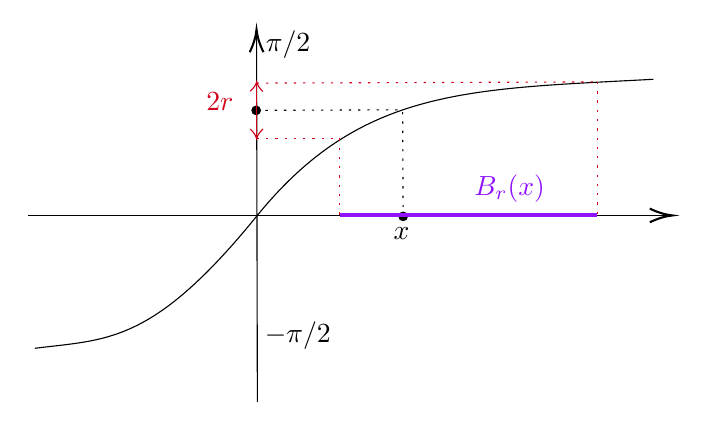
\begin{tikzpicture}[x=0.75pt,y=0.75pt,yscale=-1,xscale=1]
%uncomment if require: \path (0,300); %set diagram left start at 0, and has height of 300

%Straight Lines [id:da01253990328815191] 
\draw    (120.04,259.96) -- (119.64,82.36) ;
\draw [shift={(119.64,80.36)}, rotate = 449.87] [color={rgb, 255:red, 0; green, 0; blue, 0 }  ][line width=0.75]    (10.93,-3.29) .. controls (6.95,-1.4) and (3.31,-0.3) .. (0,0) .. controls (3.31,0.3) and (6.95,1.4) .. (10.93,3.29)   ;
%Straight Lines [id:da011511383436563216] 
\draw    (9.64,169.96) -- (318.04,169.96) ;
\draw [shift={(320.04,169.96)}, rotate = 180] [color={rgb, 255:red, 0; green, 0; blue, 0 }  ][line width=0.75]    (10.93,-3.29) .. controls (6.95,-1.4) and (3.31,-0.3) .. (0,0) .. controls (3.31,0.3) and (6.95,1.4) .. (10.93,3.29)   ;
%Curve Lines [id:da28618381116787295] 
\draw    (12.84,233.96) .. controls (48.04,229.56) and (69.64,231.96) .. (119.84,170.16) .. controls (170.04,108.36) and (221.64,109.16) .. (310.84,104.36) ;
%Flowchart: Connector [id:dp9476639517392225] 
\draw  [color={rgb, 255:red, 0; green, 0; blue, 0 }  ,draw opacity=1 ][fill={rgb, 255:red, 0; green, 0; blue, 0 }  ,fill opacity=1 ] (188.22,170.41) .. controls (188.22,169.27) and (189.14,168.35) .. (190.27,168.35) .. controls (191.41,168.35) and (192.33,169.27) .. (192.33,170.41) .. controls (192.33,171.54) and (191.41,172.46) .. (190.27,172.46) .. controls (189.14,172.46) and (188.22,171.54) .. (188.22,170.41) -- cycle ;
%Straight Lines [id:da5498910139535398] 
\draw  [dash pattern={on 0.84pt off 2.51pt}]  (190.27,170.41) -- (190.03,119.06) ;
%Straight Lines [id:da08701638969621106] 
\draw  [dash pattern={on 0.84pt off 2.51pt}]  (119.46,119.34) -- (190.03,119.06) ;
%Flowchart: Connector [id:dp6555579214360514] 
\draw  [color={rgb, 255:red, 0; green, 0; blue, 0 }  ,draw opacity=1 ][fill={rgb, 255:red, 0; green, 0; blue, 0 }  ,fill opacity=1 ] (117.4,119.34) .. controls (117.4,118.21) and (118.32,117.29) .. (119.46,117.29) .. controls (120.59,117.29) and (121.51,118.21) .. (121.51,119.34) .. controls (121.51,120.48) and (120.59,121.4) .. (119.46,121.4) .. controls (118.32,121.4) and (117.4,120.48) .. (117.4,119.34) -- cycle ;
\draw  [color={rgb, 255:red, 208; green, 2; blue, 27 }  ,draw opacity=1 ] (116.55,110.13) .. controls (118.29,108.59) and (119.35,107.05) .. (119.73,105.49) .. controls (120.03,107.06) and (121.02,108.66) .. (122.69,110.27) ;
\draw  [color={rgb, 255:red, 208; green, 2; blue, 27 }  ,draw opacity=1 ] (122.72,128.32) .. controls (121.03,129.91) and (120.02,131.49) .. (119.69,133.06) .. controls (119.34,131.49) and (118.3,129.93) .. (116.58,128.37) ;
%Straight Lines [id:da9623317046092172] 
\draw [color={rgb, 255:red, 208; green, 2; blue, 27 }  ,draw opacity=1 ]   (119.74,106.2) -- (119.74,132.77) ;
%Straight Lines [id:da5692143185430627] 
\draw [color={rgb, 255:red, 208; green, 2; blue, 27 }  ,draw opacity=1 ] [dash pattern={on 0.84pt off 2.51pt}]  (119.74,106.2) -- (283.74,105.63) ;
%Straight Lines [id:da3833790960774164] 
\draw [color={rgb, 255:red, 208; green, 2; blue, 27 }  ,draw opacity=1 ] [dash pattern={on 0.84pt off 2.51pt}]  (119.74,132.77) -- (159.74,132.77) ;
%Straight Lines [id:da40448441432128335] 
\draw [color={rgb, 255:red, 208; green, 2; blue, 27 }  ,draw opacity=1 ] [dash pattern={on 0.84pt off 2.51pt}]  (159.74,132.77) -- (159.74,169.63) ;
%Straight Lines [id:da7356169743390866] 
\draw [color={rgb, 255:red, 208; green, 2; blue, 27 }  ,draw opacity=1 ] [dash pattern={on 0.84pt off 2.51pt}]  (283.74,105.63) -- (283.74,169.63) ;
%Straight Lines [id:da876719564866242] 
\draw [color={rgb, 255:red, 144; green, 19; blue, 254 }  ,draw opacity=1 ][line width=1.5]    (159.74,169.63) -- (283.74,169.63) ;

% Text Node
\draw (122.84,79.76) node [anchor=north west][inner sep=0.75pt]   [align=left] {$\displaystyle \pi /2$};
% Text Node
\draw (122.34,219.76) node [anchor=north west][inner sep=0.75pt]   [align=left] {$\displaystyle -\pi /2$};
% Text Node
\draw (94.17,109.49) node [anchor=north west][inner sep=0.75pt]   [align=left] {$\displaystyle \textcolor[rgb]{0.82,0.01,0.11}{2r}$};
% Text Node
\draw (184.46,174.34) node [anchor=north west][inner sep=0.75pt]   [align=left] {$\displaystyle x$};
% Text Node
\draw (223.31,149.2) node [anchor=north west][inner sep=0.75pt]   [align=left] {$\displaystyle \textcolor[rgb]{0.56,0.07,1}{B_{r}( x)}$};


\end{tikzpicture}

                    \caption{Пример $B_r(x)$.}
                    \label{fig:lect11:atan_ball}
                \end{figure}

                Если $x=+\infty$, то $\exists a\in\R:\: [a,\,+\infty]\subset U\Rightarrow\forall q\in(a,\,+\infty),\, q\in\Q:\:
                    [q,\, +\infty]\subset U$.

            \end{proof}
        \end{lemma}

        Теперь докажем, что $\forall p,\, q\in \overline{\Q}$ выполнено $[p,\, q]\in\sigma(\CG)$.
        Заметим, что $[p,\, q]=[p,\, +\infty]\cap[-\infty,\, q]$. Далее
        \[
            \forall p\in\overline{\Q}\quad [p,\, +\infty]=\oR\setminus\underbrace{[-\infty,\, p)}_{U_p\in\CG}
            \in\sigma(\CG).
        \]

        Теперь докажем, что $\forall q\in\overline{\Q}\ [-\infty,\, q]\in\sigma(\CG)$:
        \begin{enumerate}
            \item[а)] Если $q=+\infty$~--- очевидно.
            \item[б)] Пусть $q\in\R$, тогда
                  \[
                      [-\infty,\, q]=\bigcap_{n\in\N}\underbrace{\left[-\infty,\, q+\dfrac{1}{n}\right)}_{U_{q+1/n}\in\CG}\in\sigma(\CG).
                  \]
            \item[в)] Если $q=-\infty$, то
                  \[
                      [-\infty,\, \infty]=\{-\infty\}=\bigcap_{n\in\N}\underbrace{[-\infty,\, -n)}_{U_{-n}\in\CG}\in\sigma(\CG).
                  \]
        \end{enumerate}

        Итак, $[p,\, q]\in\sigma(\CG)\ \forall p,\,q\in\overline{\Q}$.
        В силу леммы, для любого открытого $U\in\tau_{\oR}$ существует множество рациональных отрезков, которые в объединении дают $U$:
        \[
            \exists\left\{(p_n,\, q_n)\in\overline{\Q}^2\right\}_{n\in\N}:\quad U=\bigcup_{n=1}^{\infty}\underbrace{[p_n,\, q_n]}_{\in\sigma(\CG)}.
        \]
        В самом деле, из леммы: \[
            \forall x\in U\ \exists p_x,\, q_x\in\overline{\Q}:\: p_x<q_x\ x\in[p_x,\, q_x]\subset U\Rightarrow
            \bigcup_{x\in U}[p_x,\, q_x]=U,
        \]
        причем объединение не более чем счетно, потому как $\overline{\Q}^2$ счетно.

        Итак, получаем
        \[
            U\in\sigma(\CG)\Rightarrow\tau_{\oR}\subset\sigma(\CG)\Rightarrow
            \CB(\oR)=\sigma(\tau_{\oR})\subset\sigma(\CG).
        \]

    \end{proof}
\end{claim}

\begin{claim}
    Пусть $(X,\, \CE)$~--- измеримое пространство, $f,\, g: X\to\oR$ измеримы относительно $\CE$. Тогда
    \begin{enumerate}
        \item Для любой борелевской функции $\varphi:\:\oR\to\oR$ функция $\varphi\circ f$ измерима относительно $\CE$.
        \item Если $f$ и $g$ не принимают одновременно бесконечных значений разных знаков, то
              $\forall \alpha,\, \beta\in [0,\, +\infty)$ функция $\alpha f+\beta g$ измерима относительно $\CE$.
        \item $\min(f,\, g)$ и $\max(f,\, g)$ измеримы относительно $\CE$.
        \item $f\cdot g$ измерима относительно $\CE$.
        \item Если $g\neq 0$ и $g\neq\pm\infty$, то $\dfrac{f}{g}$ измерима относительно $\CE$.
    \end{enumerate}

    \begin{proof}

        Пусть $A\in\CB(\oR)$.

        \begin{enumerate}
            \item Распишем полный прообраз:
                  \begin{align*}
                      (\varphi\circ f)^{-1}(A) & =\{x:\: \varphi(f(x))\in A\}=                                                                               \\
                                               & =\{x:\: f(x)\in\varphi^{-1}(A)\}=                                                                           \\
                                               & =\{x:\: x\in f^{-1}(\varphi^{-1}(A))\}=f^{-1}\underbrace{\left(\varphi^{-1}(A)\right)}_{\in\CB(\oR)}\in\CE. \\
                  \end{align*}
            \item Достаточно очевидно, что умножение на константу сохраняет измеримость функции (рассмотрим случай $\alpha>0$):
                  \[
                      \{x:\: \alpha f(x)<c\}=\{x:\: f(x)< c/\alpha\}=f^{-1}(\underbrace{(-\infty,\, c/\alpha)}_{\in\CB(\oR)}).
                  \]

                  Докажем, что $f+g$ измерима.
                  Рассмотрим $N = \{x\in X:\: f(x)+g(x)>c\}$, где $c\in\R$~--- фиксированно.
                  Докажем, что $N\in\CE$.
                  Заметим, что
                  \[
                      f(x)+g(x)>c\Leftrightarrow f(x)>c-g(x)\Leftrightarrow\exists r\in\Q:\: f(x)>r,\, r > c-g(x).
                  \]
                  Следовательно, \[
                      N = \bigcup_{r\in\Q}\left(\underbrace{\{x:\: f(x)>r\}}_{\in\CE}\cap\underbrace{\{x:\:g(x)>c-r\}}_{\in\CE}\right)\in\CE.
                  \]
            \item Докажем только для минимума. Понятно, что
                  \[
                      \min(f(x),\, g(x))>c\Leftrightarrow (f(x)>c)\wedge(g(x)>c).
                  \]
                  Поэтому \[
                      \{x:\:\min(f(x),\, g(x))>c\}=\{x:\:f(x)>c\}\cap \{x:\: g(x)>c\}\in\CE.
                  \]
            \item Для начала скажем, что $f^2$~--- измерима, так как функция $\varphi(y)=y^2$~--- борелевская (см. пункт 1). А далее замечаем, что
                  \[
                      f\cdot g = \dfrac{1}{2}\left((f+g)^2-f^2-g^2\right).
                  \]
        \end{enumerate}

    \end{proof}
\end{claim}